La pluralité des mondes est un concept qui a lentement évolué au cours des âges. Dans l'antiquité grecque l'univers fini, sphérique et géocentrique d'Aristote (384--322 av. JC) s'oppose à l'univers infini et discontinu des atomistes. Pour Épicure (v 342--270 av JC), il existe une pluralité de \textit{kosmoi}, portions de ciels contenant les corps célestes. Thalès (v 625-547 av. JC) pense que d'autres astres pourraient être similaires à la Terre. 

Le débat de la vie ailleurs et de l'existence d'autres planètes autour d'autres étoiles a animé la communauté scientifique
depuis l'antiquité. Souvent influencé par les convictions religieuses et les modèles du système solaire en vigueur, il était
parfois même dangereux d'émettre l'hypothèse que d'autres planètes ou d'autres formes de vies puissent exister, l'idée de la
pluralité des civilisations étant indissociable de la question de la pluralité des mondes physiques. 

\begin{quote}
\og mesmes n'y auroit-il pas de l'apparence à croire que chaque globe est un monde, \& que tout autant qu'ils sont ce sont autant de mondes, comme autant de fiefs qui relevent de l'Empire Divin, \& eternel, assis dans la vaste estenduë du Ciel etherée, par le moyen duquel estans liez, comme par un lien commun, ils demeurent suspendus, \& que la vaste estenduë de l'Univers est composée de toutes ces differentes natures?\fg 

--- Jean d'Espagnet, \textit{La Philosophie naturelle restablie en sa pureté}, 1651, p. 241 \cite{espagnet1651philosophie}
\end{quote}

Ces questions ont longtemps été des expériences de pensées, plus philosophiques et métaphysiques qu'étayées par de quelconques observations. La découverte progressive du système solaire et de la diversité des planètes qui la compose a permis de situer la Terre dans un contexte un peu plus large. La question de la formation des planètes s'est alors posée. Remarquant la quasi coplanarité des orbites du système Solaire, Kant (1755) puis Laplace (1796) ont introduit le concept de nébuleuse solaire primitive, disque de matière duquel les planètes étaient issues. 

La ligne des glaces, séparation imaginaire au delà de laquelle l'eau est sous forme solide, s'intégrait bien dans ce concept et dans le cas du système Solaire. Pas beaucoup de matière en dessous de la ligne des glaces, nous formons des planètes essentiellement rocheuses, peu massives. Au delà, la quantité de matière augmente, nous formons des géantes gazeuses. Durant leur formation, les planètes n'évoluent pas beaucoup. La Nébuleuse Solaire de Masse Minimale (MMSN) a ainsi été inventée. Elle représente le disque le moins moins massif qui est nécessaire pour former les planètes du système Solaire. Pour cela, la masse de chaque planète est répartie sur un anneau de matière afin de remplir tout l'espace interplanétaire par de la matière. Cette masse est corrigée pour tenir compte du gaz (abondant dans le cas de géantes comme Jupiter, mais rare pour une planète comme la Terre). On obtient donc un profil de densité de surface en loi de puissance $\Sigma(R)=1700 * R^{-\sfrac32}$ \citep{
weidenschilling1977distribution, hayashi1981structure}.

La découverte de la première exoplanète\footnote{Planète orbitant autour d'une étoile autre que notre Soleil.} \citep{wolszczan1992planetary} a quelque peu bouleversé le cadre théorique de la formation planétaire.

Bien que cette dernière fut découverte en 1992, c'est en 1995 avec \object{51 Peg b} \citep{mayor1995jupiter} que la chasse aux exoplanètes a véritablement commencé. Cette planète a ceci de particulier qu'elle est semblable à Jupiter, mais plus proche de son étoile que ne l'est Mercure dans notre système. Elle orbite son étoile en $4.2$ jours. Le modèle alors en vigueur pour former les planètes était mis en défaut. Aucun modèle ne permettait de former une telle planète. 

Des travaux théoriques ont alors montré que la migration planétaire via interaction de la planète avec le disque de gaz pouvait expliquer la présence d'une géante gazeuse très proche de son étoile. Cette idée de la migration planétaire a depuis été raffinée et a même permis d'élaborer de nouvelles hypothèses sur la formation et l'évolution du système solaire. En particulier le modèle du \og Grand Tack\fg \citep{morbidelli2007dynamics, pierens2011twophase}, dans lequel Jupiter et Saturne migrent séparément vers l'intérieur, sont capturés en résonance puis migrent de concert vers l'extérieur, pouvant expliquer par la même occasion la masse étonnamment petite de Mars \citep{walsh2011low}. 

Depuis, multipliant les campagnes d'observations, les missions dédiées et les techniques de détection, on arrive, 20 ans après la première découverte à un catalogue d'exoplanètes toujours plus fourni, montrant une population extrêmement riche et variée. 939 exoplanètes ont été à ce jour observées (14 août ; \url{http://exoplanet.eu/}), apportant toujours plus de contraintes aux modèles de formation planétaire. 

Compte tenu de la difficulté à détecter les exoplanètes en raison de leur faible masse et luminosité, un premier constat s'impose : ce ne sont pas des objets rares. Si auparavant on pouvait encore en douter, il ne fait aujourd'hui plus aucun doute que les planètes sont des objets communs. C'est d'autant plus flagrant quand on note que la grande majorité des exoplanètes détectées l'ont été autour d'étoiles à moins de 400 pc du Soleil comme illustré dans \reffig{fig:milky_way_exoplanet}. 

\begin{figure}[htbp]
\centering
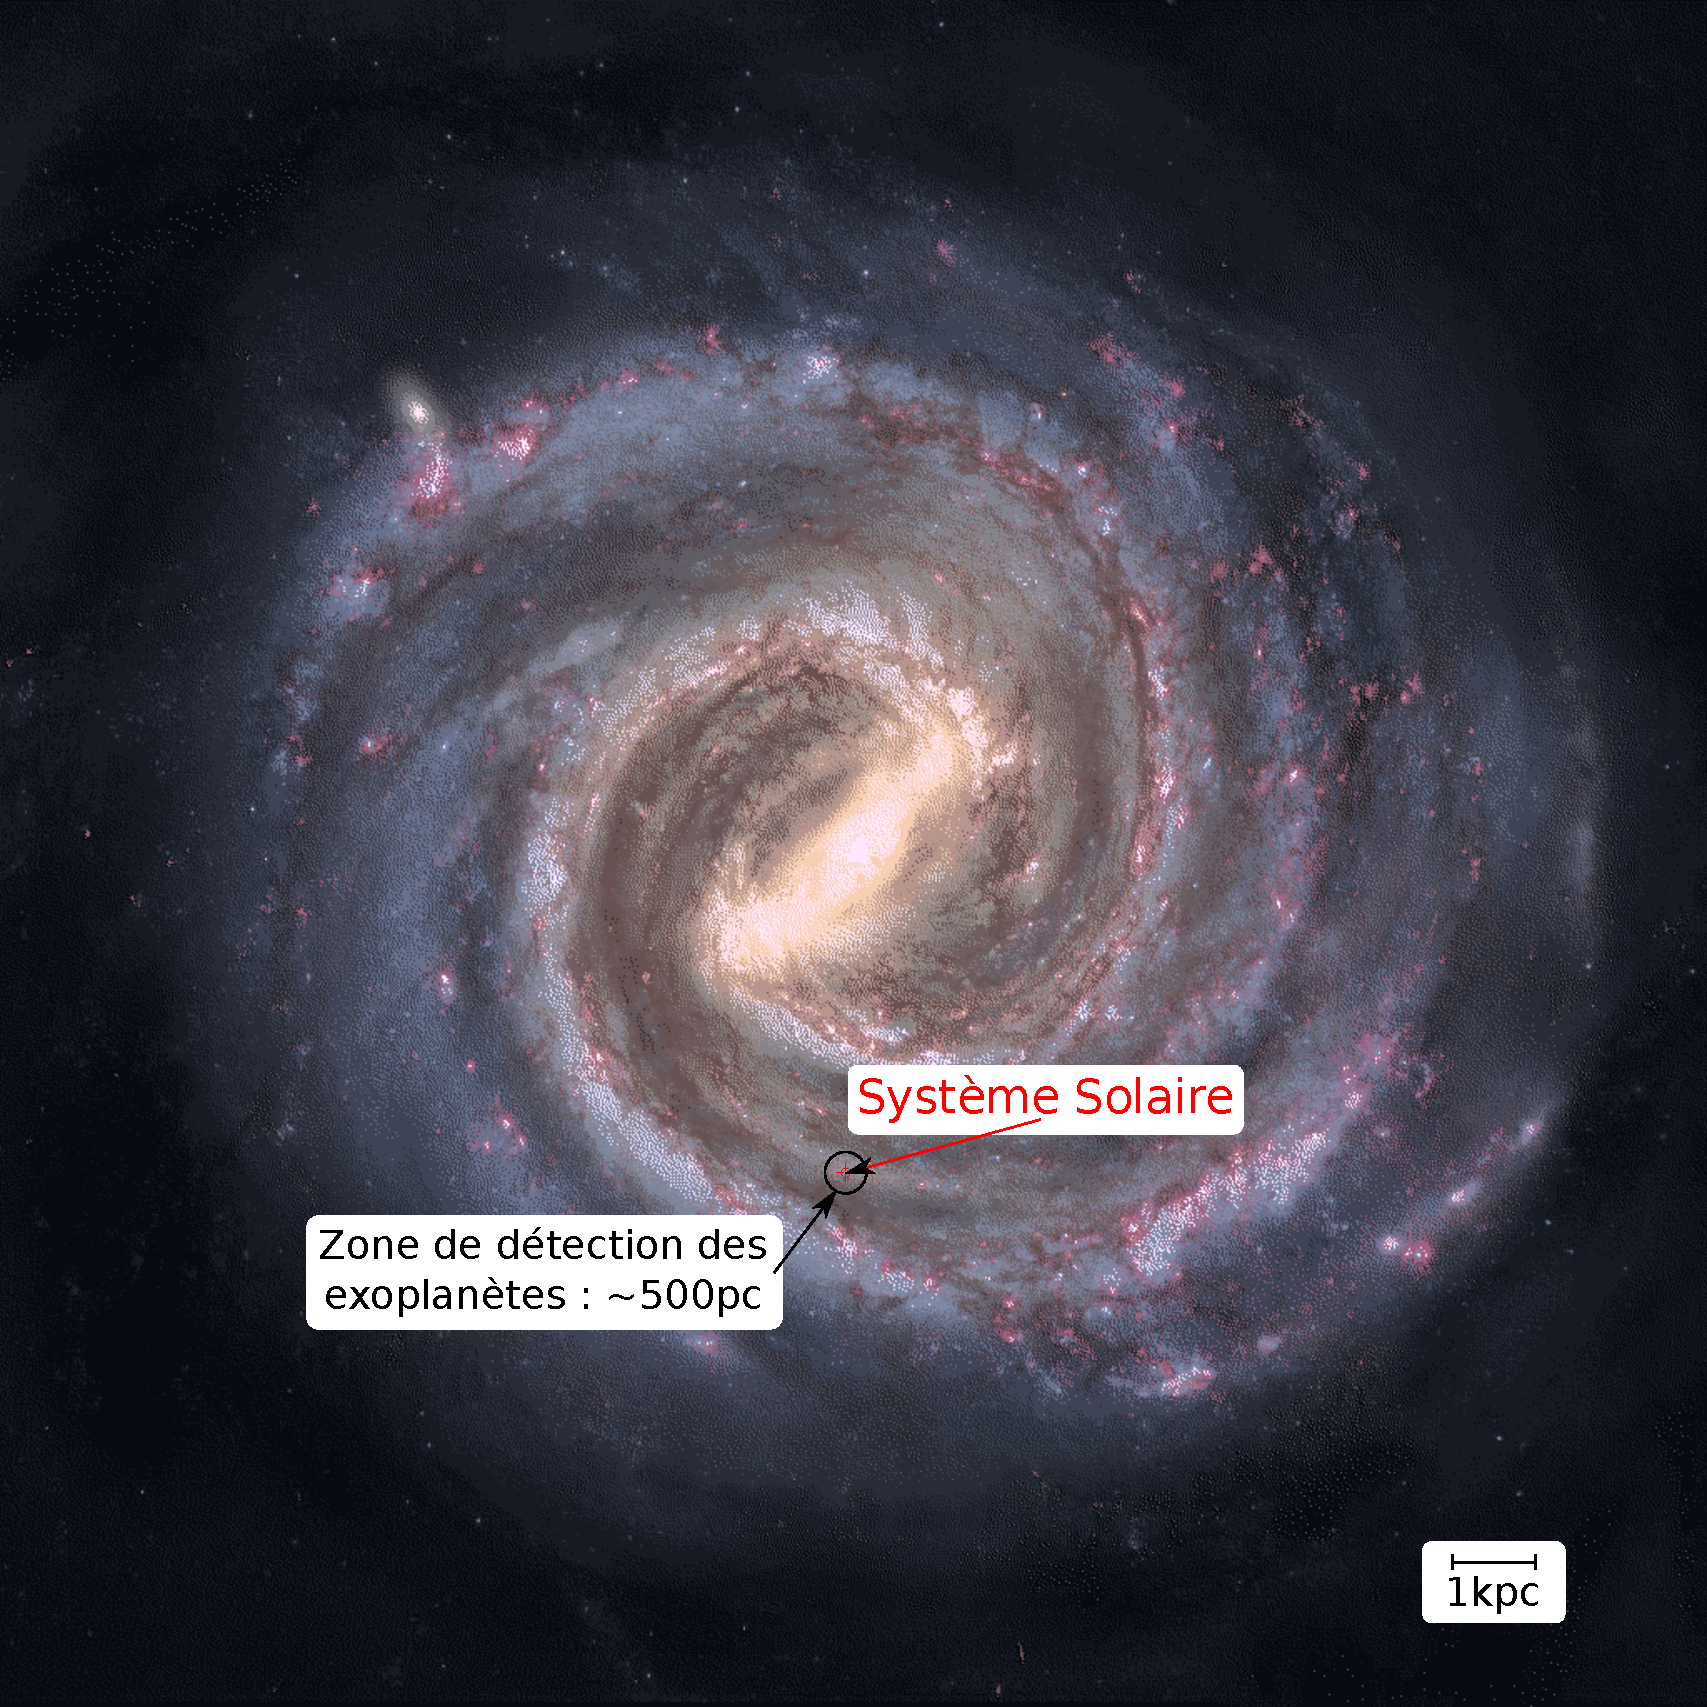
\includegraphics[width=0.45\linewidth]{figure/milky_way_exoplanets.pdf}
\caption{Image de la voie lactée avec indication de la position approximative du système solaire ainsi que de la zone (en noir) contenant la majorité des exoplanètes détectées à ce jour.}\label{fig:milky_way_exoplanet}
\end{figure}


En multipliant les méthodes de détections et les instruments, et surtout en ayant de plus en plus de planètes, il devient possible d'estimer la probabilité pour qu'une étoile héberge au moins une planète \citep{mayor2011road}. D'autres études estiment même la sensibilité de cette fréquence d'occurrence en fonction de paramètres stellaires \citep{fischer2005planet, johnson2007new, howard2012occurrence} ou planétaires \citep{mayor2011road, howard2010occurrence}. 

Mais le point qui me semble le plus intéressant est la découverte de types de planètes qui n'existent pas dans le système solaire. En un mot : diversité. Que ce soient les Jupiters chauds, comme \object{51 Peg b} ou les super-Terres comme \object{Gliese 1214 b}, ces planètes n'ont pas d'équivalent dans le système solaire. Ces variétés de composition, de taille, de systèmes nous offrent un champ de connaissance toujours plus grand dans lequel tester nos modèles de formations planétaire. Ils nous permettent aussi de mieux comprendre notre propre système, comment il s'est formé, et surtout de le mettre en perspective par rapport à tous les autres systèmes planétaires que nous observons maintenant.

Ma thèse s'inscrit dans ce cadre toujours changeant, où de nouvelles planètes viennent sans cesse remettre en cause les modèles de formation. Un type particulier de planète aura aiguisé mon intérêt en particulier, ce sont les super-Terres ($1$ - $10\mearth$). Déjà parce qu'elles sont rocheuses, à la fois semblables et différentes de la Terre, mais aussi et surtout parce qu'il n'en existe pas dans le système Solaire. Mon but a donc été d'imaginer des modèles dans lesquels la formation du système Solaire et des super-Terres serait compatible, au sein d'un même cadre théorique.

Dans un premier chapitre \refsec{sec:chap1}, je vais présenter la physique des disques, à la fois la formation et l'évolution d'un disque protoplanétaire, mais aussi les interactions entre ce dernier et les planètes qui se forment en son sein. Ensuite, je présenterai les modèles numériques que j'ai utilisé \refsec{sec:chap2}. Puis je détaillerai la migration planétaire dans une grande variété de disques protoplanétaires \refsec{sec:chap3}, variant divers paramètres clés afin d'en étudier l'influence sur la migration. Je présenterai des mécanismes de formation planétaire \refsec{sec:chap4}, en portant une attention particulière aux super-Terres. Enfin je conclurai en récapitulant les résultats principaux de ma thèse et les perspectives qui en découlent \refsec{sec:discussion}.
